% !TeX program = pdfLaTeX
\documentclass[12pt]{article}
\usepackage{amsmath}
\usepackage{graphicx,psfrag,epsf}
\usepackage{enumerate}
\usepackage{natbib}
\usepackage{textcomp}
\usepackage[hyphens]{url} % not crucial - just used below for the URL
\usepackage{hyperref}
\providecommand{\tightlist}{%
  \setlength{\itemsep}{0pt}\setlength{\parskip}{0pt}}

%\pdfminorversion=4
% NOTE: To produce blinded version, replace "0" with "1" below.
\newcommand{\blind}{0}

% DON'T change margins - should be 1 inch all around.
\addtolength{\oddsidemargin}{-.5in}%
\addtolength{\evensidemargin}{-.5in}%
\addtolength{\textwidth}{1in}%
\addtolength{\textheight}{1.3in}%
\addtolength{\topmargin}{-.8in}%

%% load any required packages here



% Pandoc citation processing

\usepackage{float}
\usepackage{mathtools}
\usepackage{natbib}
\usepackage[linesnumbered,ruled,vlined]{algorithm2e}
\usepackage{verbatim}
\usepackage{amsthm}
\usepackage{comment}
\usepackage{amsfonts}

\begin{document}


\def\spacingset#1{\renewcommand{\baselinestretch}%
{#1}\small\normalsize} \spacingset{1}


%%%%%%%%%%%%%%%%%%%%%%%%%%%%%%%%%%%%%%%%%%%%%%%%%%%%%%%%%%%%%%%%%%%%%%%%%%%%%%

\if0\blind
{
  \title{\bf Manifold Clustering in the Generalized Random Dot Product
Graph}

  \author{
        John Koo \\
    Department of YYY, University of XXX\\
      }
  \maketitle
} \fi

\if1\blind
{
  \bigskip
  \bigskip
  \bigskip
  \begin{center}
    {\LARGE\bf Manifold Clustering in the Generalized Random Dot Product
Graph}
  \end{center}
  \medskip
} \fi

\bigskip
\begin{abstract}
The text of your abstract. 200 or fewer words.
\end{abstract}

\noindent%
{\it Keywords:} block models, community detection, coordinate descent,
latent structure models, manifold clustering, random dot product graph
\vfill

\newpage
\spacingset{1.45} % DON'T change the spacing!

\newcommand{\diag}{\mathrm{diag}}
\newcommand{\tr}{\mathrm{Tr}}
\newcommand{\blockdiag}{\mathrm{blockdiag}}
\newcommand{\indep}{\stackrel{\mathrm{ind}}{\sim}}
\newcommand{\iid}{\stackrel{\mathrm{iid}}{\sim}}
\newcommand{\Bernoulli}{\mathrm{Bernoulli}}
\newcommand{\Betadist}{\mathrm{Beta}}
\newcommand{\BG}{\mathrm{BernoulliGraph}}
\newcommand{\Uniform}{\mathrm{Uniform}}
\newcommand{\PABM}{\mathrm{PABM}}
\newcommand{\RDPG}{\mathrm{RDPG}}
\newcommand{\GRDPG}{\mathrm{GRDPG}}
\newcommand{\Multinomial}{\mathrm{Multinomial}}
\newtheorem{theorem}{Theorem}
\newtheorem{lemma}{Lemma}
\newtheorem{proposition}{Proposition}
\theoremstyle{remark}
\newtheorem{remark}{Remark}
\theoremstyle{definition}
\newtheorem{definition}{Definition}
\newtheorem{example}{Example}
\newcommand{\dd}{\mathrm{d}}
\newcommand{\as}{\stackrel{\mathrm{a.s.}}{\to}}
\newcommand{\ER}{\text{Erd\"{o}s-R\'{e}nyi}}

\hypertarget{introduction}{%
\section{Introduction}\label{introduction}}

We define a \emph{Bernoulli graph} as a random graph model for which
edge probabilities are contained in an edge probability matrix
\(P \in [0, 1]^{n \times n}\), and an edge occurs between vertices \(i\)
and \(j\) with probability \(P_{ij}\). Common random graph models then
impose structure on \(P\), based on various assumptions about the way in
which the data are generated, or to allow \(P\) to be estimated. One
example is the \(\text{Erd\"{o}s-R\'{e}nyi}\) model, in which all edge
probabilities are fixed, i.e., \(P_{ij} = p\).

One common analysis task for graph and network data is community
detection, which assumes that each vertex of a graph has a hidden
community label. The goal of the analysis is then to retrieve these
labels. In order to perform this analysis as a statistical inference
task is to define a probability model with inherent community structure.
We call such models \emph{block models}: First, each vertex is assigned
a label \(z_1, ..., z_n \in \{1, 2, ..., K\}\) where \(K \ll n\). Then
each edge probability \(P_{ij}\) is said to depend on the labels \(z_i\)
and \(z_j\), possibly along with some other parameters. For example, the
stochastic block model (SBM) sets a fixed edge probability for each pair
of communities, i.e., \(P_{ij} = \omega_{z_i, z_j}\). The
degree-corrected block model (DCBM) assigns an additional parameter
\(\theta_i\) to each vertex by which edge probabilities are scaled,
i.e., \(P_{ij} = \theta_i \theta_j \omega_{z_i, z_j}\). The popularity
adjusted block model (PABM) assigns \(K\) parameters to each vertex
\(\lambda_{i1}, \lambda_{i2}, ..., \lambda_{iK}\) that describe that
vertex's affinity toward each community; the edge probability between
vertices \(i\) and \(j\) is then defined as the product of vertex
\(i\)'s affinity toward vertex \(j\)'s community and vertex \(j\)'s
affinity toward vertex \(i\)'s community, i.e.,
\(P_{ij} = \lambda_{i z_j} \lambda_{j z_i}\).

The three block model types, as well as the
\(\text{Erd\"{o}s-R\'{e}nyi}\) model, impose structure on \(P\),
including on the rank of \(P\). \(P\) has rank 1 for the
\(\text{Erd\"{o}s-R\'{e}nyi}\) model, rank \(K\) for the SBM and DCBM,
and rank \(K^2\) for the PABM. This provides the intuition behind
another family of Bernoulli graphs called the \emph{random dot product
graph} (RDPG) and \emph{generalized random dot product graph} (GRDPG).
In the RDPG, each vertex has a corresponding latent vector in
\(d\)-dimensional Euclidean space, where \(d\) is the rank of \(P\) and
\(P\) is positive semidefinite. Then the edge probability between each
pair of vertices is defined as the inner product between the
corresponding latent vectors, i.e., \(P_{ij} = x_i^\top x_j\). If the
latent vectors are collected in a data matrix
\(X = \bigl[ x_1 \mid \cdots \mid x_n \bigr]^\top\), then the edge
probability matrix for the RDPG is \(P = X X^\top\). Similarly, the edge
probability between each pair of vertices for the GRDPG is defined as
the indefinite inner product between the corresponding latent vectors,
i.e., \(P_{ij} = x_i^\top I_{p,q} x_j\), where
\(I_{p,q} = \mathrm{blockdiag}(I_p, -I_q)\) and \(p + q = d\). Then the
edge probability matrix for the GRDPG is \(P = X I_{p,q} X^\top\). This
allows for a model similar to the RDPG for non-positive semidefinite
\(P\). While the RDPG and GRDPG do not necessarily have community
structure, it has been shown that block models are specific cases of the
RDPG or GRDPG in which latent vectors are organized by community. This
includes the SBM, in which communities correspond to point masses, DCBM,
in which communities correspond to line segments, and PABM, in which
communities correspond to orthogonal subspaces. In this work, we extend
this idea to communities organized into more general latent structures.
In particular, we assume that each community corresponds to a manifold
in the latent space.

\hypertarget{latent-structure-block-models}{%
\section{Latent Structure Block
Models}\label{latent-structure-block-models}}

All block models are latent structure models.

\begin{definition}[Manifold block model]
Let $p, q \geq 0$, $d = p + q \geq 1$, $K \geq 1$, and $n \geq 1$ be integers.
If there are manifolds $\mathcal{M}_1, ..., \mathcal{M}_K \subset \mathcal{X}$ for $\mathcal{X} = \{x, y \in \mathbb{R}^d : x^\top I_{p,q} y \in [0, 1] \}$, and 
$X = \begin{bmatrix} x_1 & \cdots & x_n \end{bmatrix}^\top$ such that each $x_i \in \mathcal{M}_k$ for some $k \in [K]$, then $A \sim \mathrm{GRDPG}_{p,q}(X; \rho_n)$ is a \emph{manifold block model}.
\end{definition}

In practice, we define each manifold \(\mathcal{M}_k\) by a continuous
function \(g_k : [0, 1]^r \to \mathcal{X}\), where \(1 \leq r < d\) is
the dimensionality of manifold \(\mathcal{M}_k\).

Insert something about ASE and its consistency here.

\begin{example}
Let $p = 2$, $q = 0$, $K = 2$, and $r = 1$. 
Define two manifolds by $f_1(t) = \begin{bmatrix} \cos(\frac{\pi}{3} t) & \sin(\frac{\pi}{3} t) \end{bmatrix}^\top$ and $f_2(t) = \begin{bmatrix} 1 - \cos(\frac{\pi}{3} t) & 1 - \sin(\frac{\pi}{3} t) \end{bmatrix}^\top$.
Draw $t_1, ..., t_n \sim \mathrm{Uniform}(0, 1)$ and $z_1, ..., z_n \stackrel{\mathrm{iid}}{\sim}\mathrm{Multinomial}(\frac{1}{2}, \frac{1}{2})$, and compute latent vectors $x_i = f_{z_i}(t_i)$, which are collected in data matrix $X = \begin{bmatrix} x_1 & \cdots & x_n \end{bmatrix}^\top$. 
Finally, let $A \sim \mathrm{RDPG}(X)$. 

\begin{figure}[H]

{\centering 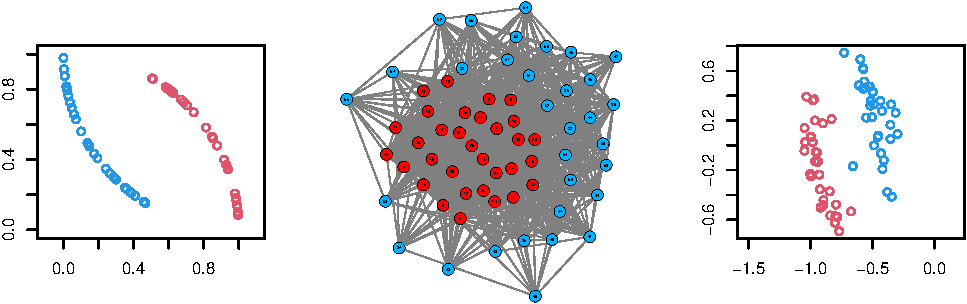
\includegraphics{draft_files/figure-latex/fig1-1} 

}

\caption{Manifold block model described in Example 1. The latent configuration is on the left, and a random dot product graph drawn from the latent configuration is on the middle, and the ASE is on the right.}\label{fig:fig1}
\end{figure}
\end{example}

\hypertarget{methods}{%
\section{Methods}\label{methods}}

Here, we provide two algorithms for MBM community detection. First, we
consider the case in which communities correspond to manifolds in the
latent space that do not intersect and are separated by some finite
distance. In this scenario, we use the convergence of the ASE to show
that single linkage clustering on the latent space produces a clustering
such that the total number of misclustered vertices goes to zero, with
high probability.

Next, we consider the case in which communities correspond to
one-dimensional manifolds in the latent space and may or may not
intersect. In this scenario, we propose an alternating coordinate
descent algorithm that alternates between estimating the structure of
the manifolds and the community labels, which we call \(K\)-curves
clustering. We again use the convergence of the ASE to show that under
certain conditions, \(K\)-curves clustering produces a clustering such
that the proportion of misclustered vertices goes to zero, with high
probability.

\hypertarget{nonintersecting-manifolds}{%
\subsection{Nonintersecting Manifolds}\label{nonintersecting-manifolds}}

In this section, we consider the following scenario: Suppose that each
community is represented by a manifold \(\mathcal{M}_k\),
\(k \in \{1, ..., K\}\) in the latent space of a RDPG or GDRPG, and the
manifolds do not intersect each other. Define
\(\delta = \min\limits_{k, \ell} \min\limits_{x \in \mathcal{M}_k, y \in \mathcal{M}_\ell} \|x - y\|\),
the minimum distance between two manifolds. We assume that
\(\delta > 0\).

First, we consider the case in which each
\(\mathcal{M}_k \subset \mathbb{R}^d\) is a one-dimensional manifold,
which can be characterized by a function
\(g_k : [0, 1] \to \mathcal{M}_k\). Let \(F\) be a probability
distribution with support \([0, 1]\). Then we define a mixture model as
follows:

\begin{enumerate}
\def\labelenumi{\arabic{enumi}.}
\tightlist
\item
  Draw \(t_1, ..., t_n \stackrel{\mathrm{iid}}{\sim}F\).
\item
  Draw
  \(z_1, ..., z_n \stackrel{\mathrm{iid}}{\sim}\mathrm{Multinomial}(\alpha_1, ..., \alpha_K)\),
  the community labels.
\item
  Let each \(x_i = g_{z_i}(t_i)\) be the latent vector for vertex
  \(v_i\).\\
  Assume
  \(\min_{k, \ell} \min_{t, s} \|g_k(t) - g_\ell(s)\| = \delta > 0\).
\item
  Draw \(A \sim \mathrm{RDPG}(X)\) or
  \(A \sim \mathrm{GRDPG}_{p,q}(X)\).
\end{enumerate}

\begin{theorem}[Community detection for one-dimensional nonintersecting manifolds without noise]
\label{nonintersect-no-noise}
Let $x_1, ..., x_n$ be points sampled on $K$ one-dimensional manifolds $\mathcal{M}_1, ..., \mathcal{M}_K$, defined by arc-length parameterizations $g_1, ..., g_K$. 
Suppose $\delta = \min_{k, \ell} \min_{t, s} \| g_k(t) - g_\ell(s) \| > 0$. 
Let $A_n$ be the event such that $\max_k \max_i \|x_{(i+1)}^{(k)} - x_{(i)}^{(k)}\| > \delta$, where $x_{(i)}^{(k)}$ is the $i^{th}$ order statistic on the $k^{th}$ manifold. 
Then for any $\epsilon > 0$, there exists an $N \in \mathbb{N}$ such that when $n > N$, $P(A_n) < \epsilon$. 
\end{theorem}

\begin{theorem}[Community detection for one-dimensional nonintersecting manifolds with noise]
\label{nonintersect-with-noise}
Suppose the same setup as in Theorem \ref{nonintersect-no-noise}. 
Define $y_i = x_i + e_i$ and $B_n$ as the event such that $\|y_{(i+1)}^{(k)} - y_{(i)}^{(k)}\| > \|y_{(i)}^{(k)} - y_{(j)}^{(\ell)}\|$ for some $i$, $j$, $k$, and $\ell$. 
Then if $\max_i \|e_i\| < \delta / 3$, for any $\epsilon > 0$, there exists an $N \in \mathbb{N}$ such that when $n > N$, $P(B_n) < \epsilon$. 
\end{theorem}

\begin{theorem}[Community detection for one-dimensional nonintersecting manifold block models]
\label{nonintersect-mbm}
Suppose we have the same setup as in Theorem \ref{nonintersect-no-noise}. 
Let $p, q \geq 0$ such that $p + q = d$ where $d$ is the dimension of the range of each $g_k$. 
Suppose we draw $A \sim \mathrm{GRDPG}_{p,q}(X; \rho_n)$ for some sparsity parameter $\rho_n \in (0, 1]$, and let $\hat{X}$ be the ASE of $A$. 
Then for any $\epsilon > 0$, there exists an $N \in \mathbb{N}$ such that when $n > N$, single linkage clustering produces zero community detection error with probability 1. 
\end{theorem}

\begin{algorithm}[h]
\DontPrintSemicolon
\SetAlgoLined
\KwData{Adjacency matrix $A$, number of communities $K$, embedding dimensions $p$ and $q$.}
\KwResult{Community assignments $z_1, ..., z_n \in \{1, ..., K\}$.}
Compute $\hat{X}$, the ASE of $A$ using the $p$ most positive and $q$ most negative eigenvalues and their corresponding eigenvectors.\;
Apply single linkage clustering with $K$ communities on $\hat{X}$\;
\caption{ASE clustering for nonintersecting communities.}
\end{algorithm}

\hypertarget{intersecting-manifolds}{%
\subsection{Intersecting Manifolds}\label{intersecting-manifolds}}

In this section, we again consider the setting for the RDPG or GRDPG in
which each community lies on a manifold in the latent space. However,
this time, we do not assume that the manifolds are nonintersecting.

\begin{algorithm}[h]
\DontPrintSemicolon
\SetAlgoLined
\KwData{Adjacency matrix $A$, number of communities $K$, embedding dimensions $p$, $q$, stopping criterion $\epsilon$}
\KwResult{Community assignments $1, ..., K$, curves $g_1, ..., g_K$}
Compute $X$, the ASE of $A$ using the $p$ most positive and $q$ most negative eigenvalues and their corresponding eigenvectors.\;
Initialize community labels $z_1, ..., z_n$.\;
\Repeat {the change in $\sum_k \sum_{i \in C_k} \|x_i - g_k(t_i)\|^2$ is less than $\epsilon$} {
\For {$k = 1, ..., K$} {
Define $X_k$ as the rows of $X$ for which $z_i = k$.\;
Fit curve $g_k$ and positions $t_{k_i}$ to $X_k$ by minimizing $\sum_{k_i} \|x_{k_i} - g_k(t_{k_i})\|^2$.\;
}
\For {$k = 1, ..., K$} {
Assign $z_i \leftarrow \arg\min_\ell \|x_i - g_\ell(t_i)\|^2$.\
}
}
\caption{$K$-curves clustering.}
\end{algorithm}

\begin{theorem}
\label{k-curves-clustering}
Let each $g_k$ be smooth. 
Then $K$-curves clustering converges to a stationary point of the objective, 
$\sum_k \sum_{i \in C_k} \|x_i - g_k(t_i)\|^2$.
\end{theorem}

\begin{proof}
$K$-curves clustering is a batch coordinate descent algorithm. 
Thus, in order to show that it converges to a stationary point, it is sufficient to show that each descent step decreases the objective function. 
\end{proof}

\(K\)-curves clustering assumes that the functional form of \(g_k\) is
known. The choice of \(g_k\) affects the difficulty of the algorithm. As
a balance between flexibility and ease of estimation, we consider the
case where each \(g_k\) is a Bezier polynomial of degree \(R\) with
coefficients \(p_k\). Then we have
\(g_k(t) = g(t; p_k) = \sum_{r=0}^R p_k^{(r)} \binom{R}{r} (1-t)^{R-r} t^r\).

Given \(\{t_i\}\) and \(\{z_i\}\), it is straightforward to obtain
\(\hat{p}_k = \arg\min_p \sum_{k_i} \|x_{k_i} - g_k (t_{k_i}; p)\|^2\)
\[\hat{p}_k = (T_k^\top T_k)^{-1} T_k^\top X_k,\] where \(T_k\) is an
\(n_k \times (R+1)\) matrix with rows
\(\begin{bmatrix} (1 - t_{k_i})^R & (1 - t_{k_i})^{R-1} t_{k_i} & \cdots & (1 - t_{k_i}) t_{k_i}^{R-1} & t_{k_i}^R \end{bmatrix}\).
Estimation of \(\{t_i\}\) given \(\{z_i\}\) and \(\{p_k\}\) is more
difficult. Each \(t_i\) can be estimated separately:
\begin{equation} \label{eq:min-t}
\hat{t}_i = \arg\min_t \|x_i - g(t; p_{z_i})\|^2. 
\end{equation} This is equivalent to solving
\(0 = (x_i - g(t; p_{z_i}))^\top (\dot{g}(t; p_{z_i}))\). Setting
\(c^{(s)} = \sum_{r=0}^s (-1)^{s-r} \binom{R}{r} p^{(r)}_{z_i}\) for
\(s \neq 0\) and \(c^{(0)} = p^{(0)}_{z_i} - x_i\), let
\(c = \begin{bmatrix} c^{(0)} & \cdots & c^{(R)} \end{bmatrix}^\top\).
Then solving Eq. \ref{eq:min-t} is equivalent to finding the real roots
of a polynomial with coefficients that are the sums of the reverse
diagonals of \(C D^\top\), where \(C_{ij} = c_{ij} (-1)^i \binom{R}{i}\)
and \(D_{ij} = c_{i-1,j} (-1)^{i-1} \binom{R-1}{i-1}\).

\begin{algorithm}[h]
\DontPrintSemicolon
\SetAlgoLined
\KwData{Adjacency matrix $A$, number of communities $K$, embedding dimensions $p$, $q$, stopping criterion $\epsilon$, $m_k \leq n_k$ known community assignments for each community}
\KwResult{Community assignments $1, ..., K$, curves $g_1, ..., g_K$}
Compute $X$, the ASE of $A$ using the $p$ most positive and $q$ most negative eigenvalues and their corresponding eigenvectors.\;
Fit curves $g_1, ..., g_K$ using each of the $m_1, ..., m_K$ points with known community labels by minimizing $\sum_{j=1}^{m_i} \|x_j - g_k(t_j)\|^2$.\;
Assign labels $z_1, ..., z_n$ to each $x_1, ..., x_n$ by minimizing $\|x_i - g_k(t_i)\|^2$ for $k$, holding the initial known labels constant.\; 
\Repeat {the change in $\sum_k \sum_{i \in C_k} \|x_i - g_k(t_i)\|^2$ is less than $\epsilon$} {
\For {$k = 1, ..., K$} {
Define $X_k$ as the rows of $X$ for which $z_i = k$.\;
Fit curve $g_k$ and positions $t_{k_i}$ to $X_k$ by minimizing $\sum_{k_i} \|x_{k_i} - g_k(t_{k_i})\|^2$.\;
}
\For {$k = 1, ..., K$} {
Assign $z_i \leftarrow \arg\min_\ell \|x_i - g_\ell(t_i)\|^2$, holding the known initial labels constant.\
}
}
\caption{Semi-supervised $K$-curves clustering.}
\end{algorithm}

\begin{theorem}
Let each $g(\cdot; p_k)$ be a nonintersecting Bezier polynomial of order $R$, 
and a GRDPG is drawn from vectors that lie on the curves. 
Suppose we observe the true labels of $m_k$ vertices from each community, and each $m_k > R + 1$. Suppose further that latent vectors $x_j = g(t_i; p_{z_j})$ that correspond to vertices with observed labels are such that 
Then as $n \to \infty$, the proportion of misclustered vertices from $K$-curves clustering approaches $0$ with probability $1$.
\end{theorem}

\hypertarget{examples}{%
\section{Examples}\label{examples}}

\begin{example}
Here, $K = 2$ with $g_1(t) = \begin{bmatrix} t^2 & 2 t (1 - t) \end{bmatrix}^\top$ and $g_2(t) = \begin{bmatrix} 2 t (1 - t) & (1 - t) ^ 2 \end{bmatrix}^\top$. We draw $n_1 = n_2 = 2^8$ points uniformly from each curve. 

\begin{figure}[H]

{\centering 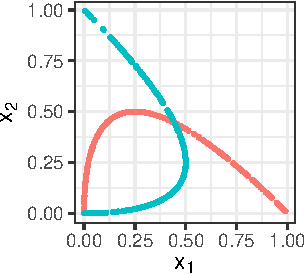
\includegraphics{draft_files/figure-latex/unnamed-chunk-2-1} 

}

\caption{Latent positions, labeled by curve/community.}\label{fig:unnamed-chunk-2}
\end{figure}

We draw $A \sim \mathrm{RDPG}(X)$ and obtain the following ASE:

\begin{figure}[H]

{\centering 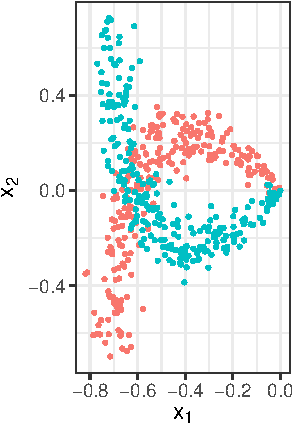
\includegraphics{draft_files/figure-latex/unnamed-chunk-3-1} 

}

\caption{ASE of an RDPG drawn from the latent positions, labeled by curve/community.}\label{fig:unnamed-chunk-3}
\end{figure}

We then try applying $K$-curves clustering to this graph. 
The first three are with random initial labels, forcing the intercept to be zero. 
The fourth initializes the labels randomly but allows the intercept to be nonzero. 
The fifth initializes the labels by spectral clustering with the normalized Laplacian, again forcing the intercept to be zero. 
The sixth also initializes via spectral clustering but allows the intercept to be nonzero. 





\begin{figure}[H]

{\centering 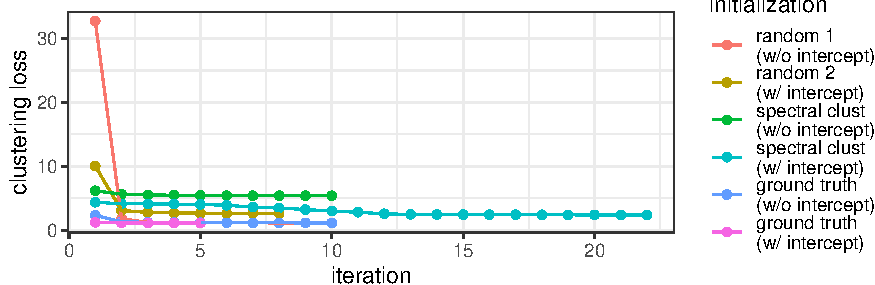
\includegraphics{draft_files/figure-latex/unnamed-chunk-6-1} 

}

\caption{Clustering loss vs. iteration for each run of K-curve clustering.}\label{fig:unnamed-chunk-6}
\end{figure}

\begin{figure}[H]

{\centering 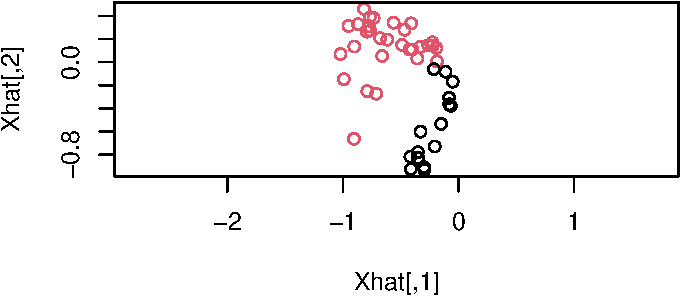
\includegraphics{draft_files/figure-latex/unnamed-chunk-7-1} 

}

\caption{ASE labeled by estimated community labels for each initialization strategy.}\label{fig:unnamed-chunk-7}
\end{figure}

\end{example}

\begin{example}[Macaque visuotactile brain areas and connections \citep{https://doi.org/10.1111/j.1460-9568.2006.04678.x}]


\begin{center}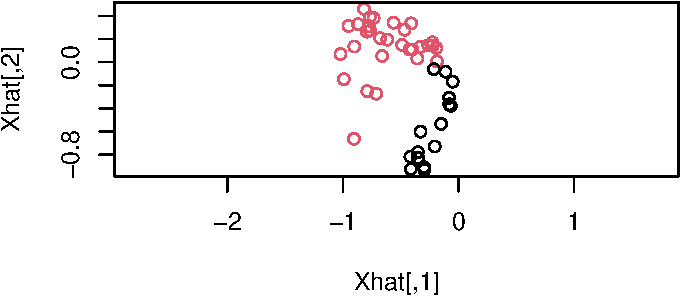
\includegraphics{draft_files/figure-latex/unnamed-chunk-8-1} \end{center}




\begin{center}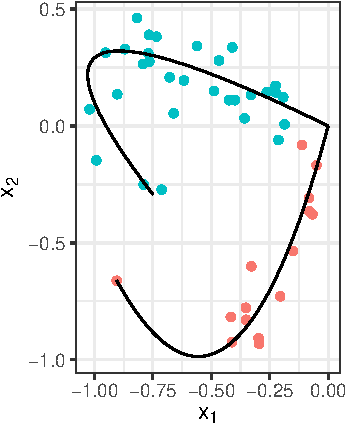
\includegraphics{draft_files/figure-latex/unnamed-chunk-10-1} \end{center}


\begin{center}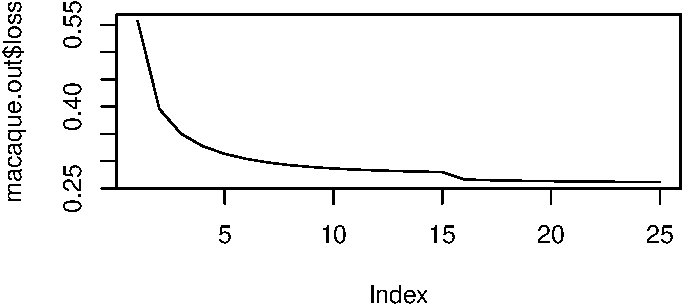
\includegraphics{draft_files/figure-latex/unnamed-chunk-11-1} \end{center}

\end{example}

\begin{example}[Non-intersecting curves]


\begin{center}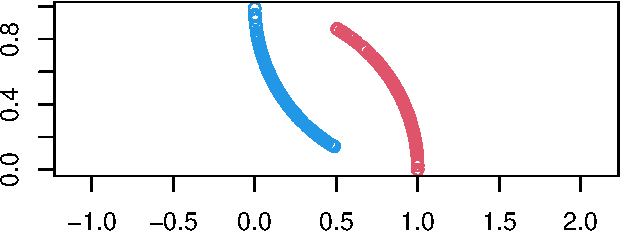
\includegraphics{draft_files/figure-latex/unnamed-chunk-12-1} \end{center}






\begin{center}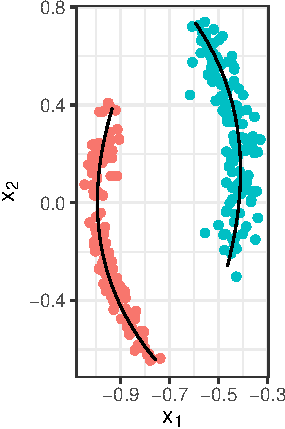
\includegraphics{draft_files/figure-latex/unnamed-chunk-15-1} \end{center}

\end{example}

\hypertarget{simulation-study}{%
\section{Simulation Study}\label{simulation-study}}

\hypertarget{discussion}{%
\section{Discussion}\label{discussion}}

\appendix

\section{Proofs of Theorems}

To prove theorems \ref{nonintersect-no-noise},
\ref{nonintersect-with-noise}, and \ref{nonintersect-mbm}, we first need
to introduce some theory for order statistics. Let
\(D_i^{(k)} = X_{(i+1)}^{(k)} - X_{(i)}^{(k)}\), where \(X_{(i)}^{(k)}\)
is the \(i^{th}\) order statistic of univariate sample
\(X_1^{(k)}, ..., X_n^{(k)} \stackrel{\mathrm{iid}}{\sim}F^{(k)}\) and
\(F^{(k)}\) is a continuous distribution on manifold \(\mathcal{M}_k\).
If \(\max_i D_i^{(k)} < \delta\), then there is sufficient separation of
points between each manifold. Then it is sufficient to quantify
\(P(\max_i D_i^{(k)} > \delta)\) for each \(k\) as a function of \(n\)
and \(\delta\) and show that this converges to zero as \(n\) grows to
\(\infty\).

For ease of notation, we drop the superscript denoting
community/manifold membership until lemma 6. Denote \(f(x)\) as the
density of each \(F\), \(g_i(x)\) as the density of \(X_{(i)}\),
\(g_{ij}(x, y)\) as the joint density of \(X_{(i)}, X_{(j)}\), and
\(h_i(d)\) as the density of \(D_i\) (with corresponding capital letters
for the cumulative distribution functions).

The following are taken as given\footnote{\url{https://en.wikipedia.org/wiki/Order_statistic}}:

\begin{enumerate}
\def\labelenumi{\arabic{enumi}.}
\tightlist
\item
  \(g_i(x) = \frac{n!}{(n-i)! (i-1)!} (F(x))^{i-1} (1 - F(x))^{n-i} f(x)\).
\item
  \(g_{ij}(x, y) = \frac{n!}{(i-1)! (j-i-1)! (n-j)!} (F(x))^{i-1} (F(y) - F(x))^{j-i-1} (1 - F(y))^{n-j} f(x) f(y)\).
\item
  By convolution,
  \(h_i(d) = \int_0^{1} g_{i, i+1} (x, x + d) \mathrm{d}x\).
\end{enumerate}

\begin{lemma}[The probability density function of $D_i$]
Suppose $X_1, ..., X_n \stackrel{\mathrm{iid}}{\sim}F$ and the support of $F$ is the unit interval. 
Let $D_i = X_{(i+1)} - X_{(i)}$. 
Then the density of each $D_i$ is: 

\begin{equation}
\label{eq:pdf}
h_i(d) = \int_0^{1-d} \frac{n!}{(i-1)! (n-i-1)!} (F(x))^{i-1} (1 - F(x+d))^{n-i-1} f(x) f(x+d) \mathrm{d}x 
\end{equation}
\end{lemma}

\begin{proof}
This is a direct consequence of 2 and 3. 
We also note that because the support of $X_i$ is $[0, 1]$, 
the integral only needs to be evaluated from $0$ to $1 - d$ 
because of the $f(x+d)$ and $1 - F(x+d)$ terms.
\end{proof}

\begin{lemma}[The cumulative distribution function of $D_i$]
Suppose $X_1, ..., X_n \stackrel{\mathrm{iid}}{\sim}F$ and the support of $F$ is the unit interval. 
Let $D_i = X_{(i+1)} - X_{(i)}$. 
Then the distribution function of each $D_i$ is:

\begin{equation}
\label{eq:cdf}
P(D_i < \delta) = H_i(\delta) = 1 - \int_0^{1-\delta} \frac{n!}{(n-i)! (i-1)!} (F(x))^{i-1} (1 - F(x + \delta))^{n-i} f(x) \mathrm{d}x
\end{equation}
\end{lemma}

\begin{proof}
$$
\begin{aligned}
H_i(\delta) & = \int_x^{x+\delta} h_i(d) \mathrm{d}d \\
& = \int_x^{x+\delta} \int_0^{1} \frac{n!}{(i-1)! (n-i-1)!} ((F(x))^{i-1} (1 - F(x+d))^{n-i-1} f(x) f(x+d) \mathrm{d}x \mathrm{d}d \\
& = \int_0^{1} \frac{n!}{(i-1)! (n-i-1)!} (F(x))^{i-1} f(x) \int_x^{x+\delta} (1 - F(x+d))^{n-i-1} f(x+d) \mathrm{d}d \mathrm{d}x \\
& = \int_0^{1} \frac{n!}{(i-1)! (n-i-1)!} (F(x))^{i-1} f(x) \int_{F(x)}^{F(x+\delta)} (1 - u)^{n-i-1} \mathrm{d}u \mathrm{d}x \\
& = \int_0^{1} \frac{n!}{(i-1)! (n-i)!} (F(x))^{i-1} f(x) ((1 - F(x))^{n-i} - (1 - F(x + \delta))^{n-i}) \mathrm{d}x \\ 
& = \int_0^1 g_i(x) \mathrm{d}x - \int_0^1 \frac{n!}{(i-1)! (n-i)!} (F(x))^{i-1} (1 - F(x + \delta))^{n-i} f(x) \mathrm{d}x \\
& = 1 - \int_0^1 \frac{n!}{(i-1)! (n-i)!} (F(x))^{i-1} (1 - F(x + \delta))^{n-i} f(x) \mathrm{d}x \\
\end{aligned}
$$

Because of the $x + \delta$ term and the fact that the support is $[0, 1]$, the integrand is zero above $1 - \delta$, so we are left with 

$$
\begin{aligned}
& = 1 - \int_0^{1 - \delta} \frac{n!}{(i-1)! (n-i)!} (F(x))^{i-1} (1 - F(x + \delta))^{n-i} f(x) \mathrm{d}x.
\end{aligned}
$$
\end{proof}

We now focus on the case where points are sampled uniformly on the unit
interval to build up to more general distributions.

\begin{lemma}[Differences between order statistics of a uniform distribution]
If $X_1, ..., X_n \stackrel{\mathrm{iid}}{\sim}\mathrm{Uniform}(0, 1)$, then each $D_i \sim \mathrm{Beta}(1, n)$.
\end{lemma}

\begin{proof}
We begin with Eq. (\ref{eq:pdf}), plugging in $f(x) = 1$ and $F(x) = x$:

$$
h_i(d) = \int_0^{1-d} \frac{n!}{(i-1)! (n-i-1)!} x^{i-1} (1-x-d)^{n-i-1} \mathrm{d}x.
$$

Then we proceed with integration by parts, setting 
$u = x^{i-1} \implies du = (i-1) x^{i-2}$ and 
$dv = (1-x-d)^{n-i-1} dx \implies v = -\frac{1}{n-i} (1-x-d)^{n-i-1}$. 
Note that $u v |_0^{1-d} = 0$ in this case. This yields

$$
= \frac{n!}{(i-1)! (n-i-1)!} \int \frac{i-1}{n-i} x^{i-2} (1-x-d)^{n-i} \mathrm{d}x.
$$

Then applying integration by parts again until the $x^p$ term disappears, we get:

$$
\begin{aligned}
& = \frac{n!}{(i-1)! (n-i-1)!} \frac{(i-1)!}{(n-i) \cdots (n-2)} \int_0^{1-d} (1-x-d)^{n-2} \mathrm{d}x \\
& = -\frac{n (n-1)}{n-1} (1-x-d)^{n-1} \Big|_0^{1-d} \\
& = n (1 - d)^{n-1}.
\end{aligned}
$$

This the density function for $\mathrm{Beta}(1, n)$, completing the proof.
\end{proof}

\begin{lemma}
Let $X_1, ..., X_n \stackrel{\mathrm{iid}}{\sim}\mathrm{Uniform}(0, 1)$. 
Then for any $\epsilon$ and $\delta > 0$, 
there exists an $N = O \big(\frac{-\log \epsilon}{\delta} \big)$ such that 
$P(\max_i X_{(i+1)} - X_{(i)} < \delta) \geq 1 - \epsilon$ when $n > N$.
\end{lemma}

\begin{proof}
Since $X_{(i+1)} - X_{(i)} = D_i \sim \mathrm{Beta}(1, n)$, 
$P(X_{(i+1)} - X_{(i)} < \delta) = 1 - (1 - \delta)^n $. This yields

$$
\begin{aligned}
P(\max_i D_i < \delta) & \geq (P(D_i < \delta))^{n-1} \\
& = (1 - (1 - \delta)^n)^{n-1} \\
& \approx e^{-n \exp(-n \delta)}.
\end{aligned}
$$

In the limit $n \to \infty$, this goes to 1.
\end{proof}

Now we extend this lemma to general distributions on the unit interval.

\begin{lemma}
\label{lem:lim-d}
Let $X_1, ..., X_n \stackrel{\mathrm{iid}}{\sim}F$ with support $[0, 1]$, and suppose $f(x)$ is continuous and $f(x) \geq a > 0$ everywhere on the support. 
Let $D_i = X_{(i+1)} - X_{(i)}$. 
Then for any $\epsilon > 0$, there exists $N > 0$ such that $P(\max_i D_i < \delta) \geq 1 - \epsilon$ when $n > N$.
\end{lemma}

\begin{proof}
We start with Eq. (\ref{eq:cdf}):

$$P(D_i \leq \delta) = 1 - \int_0^{1-\delta} \frac{n!}{(n-i)! (i-1)!} (F(x))^{i-1} (1 - F(x + \delta))^{n-i} f(x) \mathrm{d}x.$$

Making the approximation $F(x+\delta) \approx F(x) + \delta f(x)$ 
and bounding $f(x) \geq a$, we get:

$$P(D_i \leq \delta) \geq 1 - \int_0^{1-\delta} \frac{n!}{(n-i)! (i-1)!} (F(x))^{i-1} (1 - F(x) - a \delta)^{n-i} f(x) \mathrm{d}x.$$

Then making the substitution $u = F(x) \implies du = f(x) \mathrm{d}x$, we obtain 

$$1 - \int_0^{F(1-\delta)} \frac{n!}{(n-i)! (i-1)!} u^{i-1} (1 - u - a \delta)^{n-i} \mathrm{d}u$$

Evaluating the integral yields

$$P(D_i < \delta) = 1 - (1 - a \delta)^n + (1 - F(1-\delta) - a \delta)^n.$$

Then as before,

$$
\begin{aligned}
P(\max_i D_i < \delta) & = P(\text{all } D_i < \delta) \\
& = 1 - P(\text{some } D_i > \delta) \\
& \geq 1 - \sum_i^{n-1} P(D_i > \delta) \\
& = 1 - (n - 1) (1 - a \delta)^n + (n - 1) (1 - F(1 - \delta) - a \delta)^n
\end{aligned}
$$

This converges to $1$ in the limit $n \to \infty$.
\end{proof}

\begin{proof}[Proof of Theorem \ref{nonintersect-no-noise}]
For this theorem to be true, there are two additional conditions: 
First, each $n_k \to \infty$ as $n \to \infty$, or the sample size on each manifold grows with $n$, and second, the number of manifolds $K$ remains fixed. 
Then this is a direct consequence of Lemma \ref{lem:lim-d}. 
Here, we denote $m = \min_k n_k$ as the sample size of the manifold with the fewest points. 

$$
\begin{aligned}
P(\max_{k,i} \|X_{(i+1)}^{(k)} - X_{(i)}^{(k)}\| < \delta) & = P(\forall k, i ~ D_i^{(k)} < \delta) \\
& \geq \prod_{k=1}^K P(D_i^{(k)} < \delta) \\
& \geq (1 - (m-1) (1 - a \delta)^{m} + (m-1) (1 - F(1-\delta) - a \delta)^{m})^K
\end{aligned}
$$
Since as $n \to \infty$, $m \to \infty$ as well, and $K$ is fixed, this approaches $(1)^K = 1$. 
\end{proof}

Here, we extend the results on the line to the unit hypercube. The
following theorem is based on Lemma 2 of
\citet{trosset2020rehabilitating}.

\begin{lemma}
\label{thm:multidim}
Let $X_1, ..., X_n \stackrel{\mathrm{iid}}{\sim}F$ with support $[0, 1]^r$, and $f(x) \geq a > 0$ everywhere on the support. 
Define $E_n$ as the event that an $\eta$-neighborhood graph constructed from the sample is connected. 
Then for any $\epsilon > 0$, there exists $N = O \bigg( \frac{\log \epsilon \eta^r / r^{r/2}}{\log (1 - \frac{a \eta^r}{r^{r / 2}})} \bigg)$ such that $P(E_n) > 1 - \epsilon$ when $n \geq N$.
\end{lemma}

\begin{proof}[Proof (sketch)]
Divide the hypercube $[0, 1]^r$ into a grid of sub-hypercubes of side length at most $\eta / \sqrt{r}$. 
$E_n$ is satisfied if each sub-hypercube contains at least one $X_i$ from the sample. 

$$
\begin{aligned}
P(E_n) & = 1 - P(\text{some cells don't contain } X_i) \\
& \geq 1 - \sum_k^{\lceil \sqrt{r} / \eta \rceil^r} \prod_i^n P(X_i \text{ is not in the } k^{th} \text{ hypercube}) \\
& \geq 1 - \lceil \sqrt{r} / \eta \rceil^r (1 - a \eta^r / r^{r/2})^n
\end{aligned}
$$

Setting this $\geq 1 - \epsilon$ and solving for $n$ yields the desired rate. 
\end{proof}

\section{Details on Fitting Bezier Curves with Noise}

\bibliographystyle{agsm}
\bibliography{bibliography.bib}

\end{document}
